\documentclass[11pt,a4paper]{article}

\usepackage[utf8]{inputenc}
\usepackage[T1]{fontenc}
\usepackage{babel}
\usepackage{geometry}
\usepackage{amsmath}
\usepackage{amssymb}
\usepackage{booktabs}
\usepackage{array}
\usepackage{tabularx}
\usepackage{longtable}
\usepackage{listings}
\usepackage{xcolor}
\usepackage{hyperref}
\usepackage{enumitem}
\usepackage{titlesec}
\usepackage{fancyhdr}
\usepackage{graphicx}
\usepackage{parskip}

\geometry{
  top=2.5cm,
  bottom=2.5cm,
  left=2.5cm,
  right=2.5cm
}

% Colors
\definecolor{codeblue}{RGB}{0,83,156}
\definecolor{codegray}{RGB}{128,128,128}
\definecolor{codegreen}{RGB}{0,128,0}
\definecolor{backcolour}{RGB}{248,248,248}
\definecolor{darkblue}{RGB}{0,50,120}

% Listings style
\lstdefinestyle{pseudocode}{
  backgroundcolor=\color{backcolour},
  commentstyle=\color{codegreen}\itshape,
  keywordstyle=\color{codeblue}\bfseries,
  numberstyle=\tiny\color{codegray},
  stringstyle=\color{orange},
  basicstyle=\ttfamily\small,
  breakatwhitespace=false,
  breaklines=true,
  captionpos=b,
  keepspaces=true,
  numbers=left,
  numbersep=5pt,
  showspaces=false,
  showstringspaces=false,
  showtabs=false,
  tabsize=2,
  frame=single,
  framerule=0.4pt,
  rulecolor=\color{codegray}
}
\lstset{style=pseudocode}

% Hyperref setup
\hypersetup{
  colorlinks=true,
  linkcolor=darkblue,
  urlcolor=codeblue,
  citecolor=darkblue
}

% Section formatting
\titleformat{\section}{\large\bfseries\color{darkblue}}{}{0em}{\thesection.\quad}[\titlerule]
\titleformat{\subsection}{\normalsize\bfseries\color{darkblue}}{\thesubsection}{1em}{}

% Header/Footer
\pagestyle{fancy}
\fancyhf{}
\fancyhead[L]{\small LU3IN025 -- Rapport Projet}
\fancyhead[R]{\small 3\textsuperscript{ème} Projet}
\fancyfoot[C]{\thepage}
\renewcommand{\headrulewidth}{0.4pt}

% Custom commands
\newcommand{\PLNE}{\textsc{plne}}
\newcommand{\GS}{\textsc{gs}}

%---------------------------------------------------------------
\begin{document}

%---------------------------------------------------------------
% Title page
%---------------------------------------------------------------
\begin{titlepage}
  % Noms en haut à gauche
  \noindent
  {\large
    \textbf{Alexandre Hurel} \quad \textit{21231339}\\[0.2cm]
    \textbf{Mayes Haddab} \quad \textit{21206341}
  }

  \centering
  \vspace*{3cm}
  {\Huge\bfseries\color{darkblue} LU3IN025 -- Rapport Projet\par}
  \vspace{0.5cm}
  {\Large 3\textsuperscript{ème} Projet\par}
  \vspace{1cm}
  \rule{\linewidth}{0.5pt}\\[0.4cm]
  {\large\itshape Affectation stable par l'algorithme de Gale-Shapley et \PLNE\par}
  \rule{\linewidth}{0.5pt}
  \vspace{2cm}
  {\large \textbf{Fichier principal :} \texttt{projet.py}\par}
  \vfill
  {\large Sorbonne Université\par}
  {\normalsize L3 Informatique -- Année 2025--2026\par}
\end{titlepage}

\tableofcontents
\newpage

%---------------------------------------------------------------
\section{Reformulation du sujet}
%---------------------------------------------------------------

On cherche à affecter \textbf{$n = 13$ étudiants} dans \textbf{$m = 10$ parcours} du Master Informatique de Sorbonne Université (AI2D, BIM, CCA, IMA, MIND, QI, RES, SAR, SESI, STL), chaque parcours ayant une capacité d'accueil. Les deux côtés expriment des préférences ordonnées sur l'autre côté. L'objectif est de produire des \textbf{affectations stables} via l'algorithme de Gale-Shapley (côté étudiants, puis côté parcours), d'étudier leurs performances en temps et en nombre d'itérations, puis d'optimiser l'équité via la \textbf{Programmation Linéaire en Nombres Entiers (\PLNE)} avec Gurobi.

%---------------------------------------------------------------
\section{Code et structures de données}
%---------------------------------------------------------------

\subsection{Organisation du code}

\texttt{projet.py} est structuré en \textbf{7 classes} :

\begin{center}
\begin{tabular}{lll}
\toprule
\textbf{Classe} & \textbf{Questions} & \textbf{Rôle} \\
\midrule
\texttt{PreferenceData} & Q1 & Lecture de \texttt{PrefEtu.txt} / \texttt{PrefSpe.txt} ; \\
 & & construction de CE, CP et des matrices de rang \\
\texttt{GaleShapleyStudentSide} & Q2--Q3 & GS côté étudiants avec max-heap \\
\texttt{GaleShapleySpeSide} & Q4--Q5 & GS côté parcours \\
\texttt{StabilityChecker} & Q6 & Détection des paires instables en $O(n \times m)$ \\
\texttt{RandomGenerator} & Q7 & Génération d'instances aléatoires \\
\texttt{PerformanceMeasurer} & Q8--Q10 & Mesure du temps et des itérations, tracé des courbes \\
\texttt{PLNESolver} & Q11--Q14 & Formulations \PLNE{} résolues avec Gurobi \\
\bottomrule
\end{tabular}
\end{center}

\subsection{Matrices principales (Q1)}

\begin{itemize}
  \item \textbf{CE$[i]$} : liste des IDs de parcours par ordre de préférence de l'étudiant $i$ (1\textsuperscript{er} choix en tête).
  \item \textbf{CP$[j]$} : liste des IDs d'étudiants par ordre de préférence du parcours $j$.
  \item \textbf{rank\_etu$[i][j]$} : rang du parcours $j$ dans la liste de $i$ (0 = meilleur), précalculé en $O(n \times m)$.
  \item \textbf{rank\_spe$[j][i]$} : rang de l'étudiant $i$ dans la liste de $j$, précalculé en $O(n \times m)$.
\end{itemize}

Ces matrices inverses permettent des comparaisons de préférences en $O(1)$ au lieu de $O(m)$ ou $O(n)$.

\subsection{Description schématique des algorithmes}

\textbf{GS côté étudiants} (student-optimal) :

\begin{lstlisting}[language={},mathescape=true]
Initialiser : file deque de tous les etudiants libres,
              next_proposal[i] = 0 pour tout i
Tant qu'il existe un etudiant libre i :
    j <- CE[i][next_proposal[i]++]
    Si |assignment[j]| < cap_j :
        affecter i -> j  (heappush dans worst_heap[j])
    Sinon :
        w <- pire de j (sommet du max-heap : rank_spe[j][w] maximal)
        Si rank_spe[j][i] < rank_spe[j][w] :   // j prefere i a w
            remplacer w par i dans j  (heapreplace en O(log cap_j))
            w redevient libre
        Sinon : i reste libre (proposera a CE[i][next_proposal[i]])
Retourner assignment
\end{lstlisting}

\textbf{GS côté parcours} (specialty-optimal) :

\begin{lstlisting}[language={},mathescape=true]
Initialiser : active = {tous les parcours},
              next_proposal[j] = 0, current_spe[i] = None
Tant qu'il existe un parcours actif j :
    active.discard(j)
    Tant que |assignment[j]| < cap_j et next_proposal[j] < n :
        i <- CP[j][next_proposal[j]++]
        Si current_spe[i] est None :
            affecter i -> j
        Sinon (i est dans j') :
            Si rank_etu[i][j] < rank_etu[i][j'] :  // i prefere j a j'
                deplacer i de j' vers j
                Si j' sous-rempli et a des candidats restants :
                    active.add(j')
            Sinon : j continue (passe au candidat suivant)
Retourner assignment
\end{lstlisting}

%---------------------------------------------------------------
\section{Réponses aux questions}
%---------------------------------------------------------------

\subsection*{Q2 -- Structures de données pour GS côté étudiants}

\begin{center}
\begin{tabular}{lll}
\toprule
\textbf{Opération} & \textbf{Structure} & \textbf{Complexité} \\
\midrule
Trouver un étudiant libre & \texttt{deque} & $O(1)$ \\
Prochain parcours à proposer & \texttt{next\_proposal[i]} (liste) & $O(1)$ \\
Rang de $i$ dans $j$ & \texttt{rank\_spe[j][i]} (tableau 2D précalculé) & $O(1)$ \\
Pire étudiant de $j$ & \texttt{worst\_heap[j]} (max-heap via négation du rang) & $O(\log \mathrm{cap}_j)$ \\
Remplacer dans $j$ & \texttt{heapreplace} + \texttt{set.add/remove} & $O(\log \mathrm{cap}_j)$ \\
\bottomrule
\end{tabular}
\end{center}

La max-heap stocke $(-\texttt{rank\_spe}[j][i],\, i)$ : le minimum Python (sommet) correspond à l'étudiant que $j$ classe en dernier parmi ses affectés actuels.

\textbf{Occupation mémoire :} $O(n \times m)$ pour les matrices de rang, $O(n)$ pour les structures auxiliaires.

%---------------------------------------------------------------
\subsection*{Q3 -- Algorithme GS côté étudiants et complexité}

Chaque étudiant propose à au plus $m$ parcours $\Rightarrow$ au plus $n \times m$ propositions, chacune coûtant $O(\log \mathrm{cap}_{\max})$ pour les opérations de heap.

\[
  \textbf{Complexité totale : } O(n \times m \times \log(\mathrm{cap}_{\max}))
\]

Avec capacités équilibrées ($\mathrm{cap} \approx n/m$) : $O(n \times m \times \log(n/m))$.

Sur l'instance réelle : \textbf{28 propositions} (pire cas théorique : $n \times m = 130$).

%---------------------------------------------------------------
\subsection*{Q4 -- Algorithme GS côté parcours et complexité}

Chaque parcours propose à au plus $n$ étudiants $\Rightarrow$ au plus $n \times m$ propositions, chacune en $O(1)$ grâce à \texttt{rank\_etu}.

\[
  \textbf{Complexité totale : } O(n \times m)
\]
Strictement meilleure que côté étudiant lorsque $\mathrm{cap}_{\max}$ est grand.

\begin{center}
\begin{tabular}{lll}
\toprule
\textbf{Opération} & \textbf{Structure} & \textbf{Complexité} \\
\midrule
Parcours actif & \texttt{active} (set) & $O(1)$ \\
Prochain étudiant à contacter & \texttt{next\_proposal[j]} (liste) & $O(1)$ \\
Comparer deux parcours pour $i$ & \texttt{rank\_etu[i][j]} (tableau 2D) & $O(1)$ \\
Parcours actuel de $i$ & \texttt{current\_spe[i]} (liste) & $O(1)$ \\
Modifier l'affectation & \texttt{assignment[j]} (set) & $O(1)$ \\
\bottomrule
\end{tabular}
\end{center}

Sur l'instance réelle : \textbf{57 propositions}.

%---------------------------------------------------------------
\subsection*{Q5 -- Application sur les fichiers de test}

Les deux algorithmes produisent la \textbf{même affectation} (unicité de l'affectation stable sur cet exemple) :

\begin{center}
\begin{tabular}{lcc}
\toprule
\textbf{Parcours} & \textbf{Cap.} & \textbf{Étudiants affectés} \\
\midrule
AI2D & 2 & Etu5, Etu12 \\
BIM & 1 & Etu4 \\
CCA & 1 & Etu9 \\
IMA & 1 & Etu8 \\
MIND & 2 & Etu10, Etu11 \\
QI & 1 & Etu0 \\
RES & 1 & Etu1 \\
SAR & 1 & Etu7 \\
SESI & 1 & Etu6 \\
STL & 2 & Etu2, Etu3 \\
\bottomrule
\end{tabular}
\end{center}

%---------------------------------------------------------------
\subsection*{Q6 -- Vérification de la stabilité}

Une paire $(i, j)$ est instable si : $i \notin \texttt{assignment}[j]$, $i$ préfère $j$ à son affectation courante, et $j$ préfère $i$ à l'un de ses étudiants (ou $j$ a une place libre).

La méthode \texttt{StabilityChecker.find\_unstable\_pairs} procède en deux passes :
\begin{enumerate}
  \item Construire \texttt{current\_spe}$[i]$ (affectation inverse) en $O(n)$.
  \item Pré-calculer \texttt{worst\_rank\_in}$[j]$ = rang maximum parmi les étudiants de $j$, en $O(n)$ au total.
  \item Tester toutes les paires $(i, j)$ : chaque test est $O(1)$.
\end{enumerate}

\textbf{Complexité : $O(n \times m)$.}

\textbf{Résultats :}
\begin{itemize}
  \item GS côté étudiants : \textbf{0 paire instable} \checkmark
  \item GS côté parcours : \textbf{0 paire instable} \checkmark
\end{itemize}

%---------------------------------------------------------------
\subsection*{Q7 -- Génération d'instances aléatoires}

\begin{itemize}
  \item \texttt{generate\_CE(n, m)} : permutation aléatoire de $[0, m-1]$ pour chaque étudiant.
  \item \texttt{generate\_CP(n, m)} : permutation aléatoire de $[0, n-1]$ pour chaque parcours.
  \item \texttt{generate\_balanced\_capacities(n, m)} : $\mathrm{cap}_j = \lfloor n/m \rfloor$, les $n \bmod m$ premiers ont $\mathrm{cap}_j + 1$ ; garantit $\sum \mathrm{cap} = n$.
\end{itemize}

%---------------------------------------------------------------
\subsection*{Q8 -- Mesure des temps de calcul}

Résultats moyens (10 tests par valeur de $n$, $m = 10$, capacités équilibrées) :

\begin{center}
\begin{tabular}{rrrrrr}
\toprule
$n$ & $t_{\text{etu}}$ (ms) & $t_{\text{parcours}}$ (ms) & iter.\ etu & iter.\ parcours \\
\midrule
200   & 0.12 & 0.28 & 261   & 882    \\
400   & 0.15 & 0.37 & 479   & 1\,820 \\
600   & 0.22 & 0.59 & 710   & 2\,900 \\
800   & 0.29 & 0.82 & 931   & 4\,038 \\
1\,000 & 0.37 & 1.06 & 1\,126 & 5\,177 \\
1\,200 & 0.41 & 1.27 & 1\,349 & 6\,240 \\
1\,400 & 0.51 & 1.53 & 1\,571 & 7\,423 \\
1\,600 & 0.55 & 1.80 & 1\,776 & 8\,693 \\
1\,800 & 0.58 & 1.96 & 1\,966 & 9\,597 \\
2\,000 & 0.67 & 2.27 & 2\,180 & 10\,905 \\
\bottomrule
\end{tabular}
\end{center}

Courbes sauvegardées : \texttt{performance\_times.png} (temps) et \texttt{performance\_iters.png} (itérations).

%---------------------------------------------------------------
\subsection*{Q9 -- Complexité observée}

Les temps croissent \textbf{linéairement} en $n$ pour les deux algorithmes ($m = 10$ fixé), conformément à :
\begin{itemize}
  \item GS côté étudiants : $O(n \times m \times \log(n/m)) \approx O(n \log n) \approx O(n)$ pour $m$ constant.
  \item GS côté parcours : $O(n \times m) = O(n)$ pour $m$ constant.
\end{itemize}

Le ratio des temps $t_{\text{spe}}/t_{\text{etu}} \approx 3{,}4\times$ à $n = 2\,000$ s'explique directement par le ratio d'itérations $\approx 5{,}0\times$ : chaque itération côté parcours est certes en $O(1)$ (plus rapide que $O(\log \mathrm{cap})$), mais le nombre total de propositions est bien supérieur.

%---------------------------------------------------------------
\subsection*{Q10 -- Nombre d'itérations}

Les itérations croissent également \textbf{linéairement} en $n$ :
\begin{itemize}
  \item Côté étudiants : $\approx 1{,}1n$ propositions en moyenne (la plupart des étudiants trouvent rapidement une place).
  \item Côté parcours : $\approx 5{,}4n$ propositions en moyenne (phénomène analogue au problème du coupon collector : chaque parcours doit parcourir plus d'étudiants pour remplir son quota face aux refus).
\end{itemize}

À $n = 2\,000$ : côté etu $\approx 11\%$ du pire cas ($n \times m = 20\,000$), côté parcours $\approx 55\%$ -- tous deux restent bien en-deçà du pire cas théorique.

%---------------------------------------------------------------
\subsection*{Q11 -- PLNE maximisant l'utilité minimale des étudiants}

Le \textbf{score de Borda} de l'étudiant $i$ affecté au parcours $j$ est défini par :
\[
  b_{ij} = m - 1 - \texttt{rank\_etu}[i][j] \;\in\; \{0, \ldots, m-1\}.
\]

\textbf{Variables :} $x_{ij} \in \{0,1\}$ indique si l'étudiant $i$ est affecté au parcours $j$ ; $U_{\min} \geq 0$ est l'utilité minimale à maximiser.

\bigskip
\begin{equation*}
\begin{aligned}
  &\textbf{Maximiser} \quad U_{\min} \\[6pt]
  &\textbf{Sous les contraintes :} \\[4pt]
  &\quad U_{\min} \;\leq\; \sum_{j} b_{ij} \cdot x_{ij}, && \forall i \quad \text{(chaque étudiant a une utilité} \geq U_{\min}\text{)} \\[4pt]
  &\quad \sum_{j} x_{ij} = 1, && \forall i \quad \text{(chaque étudiant est affecté à exactement un parcours)} \\[4pt]
  &\quad \sum_{i} x_{ij} \leq \mathrm{cap}_j, && \forall j \quad \text{(respect de la capacité de chaque parcours)} \\[4pt]
  &\quad x_{ij} \in \{0,1\}, && \forall i, j
\end{aligned}
\end{equation*}

\textbf{Résultat Gurobi :} $U_{\min}$ optimal $= \mathbf{5}$ (vs 4 pour \GS), utilité moyenne $= 8{,}23$ ; 3 paires instables.

%---------------------------------------------------------------
\subsection*{Q12 -- PLNE maximisant la somme des utilités}

On définit le score de Borda du parcours $j$ pour l'étudiant $i$ par :
\[
  c_{ji} = n - 1 - \texttt{rank\_spe}[j][i].
\]

\bigskip
\begin{equation*}
\begin{aligned}
  &\textbf{Maximiser} \quad \sum_{i,j} (b_{ij} + c_{ji}) \cdot x_{ij} \\[6pt]
  &\textbf{Sous les contraintes :} \\[4pt]
  &\quad \sum_{j} x_{ij} = 1, && \forall i \quad \text{(chaque étudiant est affecté à exactement un parcours)} \\[4pt]
  &\quad \sum_{i} x_{ij} \leq \mathrm{cap}_j, && \forall j \quad \text{(respect de la capacité de chaque parcours)} \\[4pt]
  &\quad x_{ij} \in \{0,1\}, && \forall i, j
\end{aligned}
\end{equation*}

\textbf{Résultat Gurobi :} utilité totale $= \mathbf{213}$, utilité moyenne étudiants $= 7{,}77$, minimum $= 4$ ; 7 paires instables.

%---------------------------------------------------------------
\subsection*{Q13 -- PLNE avec contrainte des $k$ premiers choix}

Un étudiant $i$ est dans ses $k$ premiers choix si et seulement si son score de Borda vérifie :
\[
  b_{ij} \geq m - k \quad \Longleftrightarrow \quad \texttt{rank\_etu}[i][j] \leq k - 1.
\]

\bigskip
\begin{equation*}
\begin{aligned}
  &\textbf{Maximiser} \quad \sum_{i,j} (b_{ij} + c_{ji}) \cdot x_{ij} \\[6pt]
  &\textbf{Sous les contraintes :} \\[4pt]
  &\quad \sum_{j} x_{ij} = 1, && \forall i \quad \text{(chaque étudiant est affecté à exactement un parcours)} \\[4pt]
  &\quad \sum_{i} x_{ij} \leq \mathrm{cap}_j, && \forall j \quad \text{(respect de la capacité de chaque parcours)} \\[4pt]
  &\quad \sum_{j} b_{ij} \cdot x_{ij} \geq m - k, && \forall i \quad \text{(chaque étudiant est affecté dans ses $k$ premiers choix)} \\[4pt]
  &\quad x_{ij} \in \{0,1\}, && \forall i, j
\end{aligned}
\end{equation*}

%---------------------------------------------------------------
\subsection*{Q14 -- Plus petit $k$ pour un mariage parfait}

On résout Q13 pour $k = 1, 2, 3, \ldots$ jusqu'à la première faisabilité :

\begin{center}
\begin{tabular}{ccc}
\toprule
$k$ & \textbf{Faisable ?} & \textbf{Util.\ min étu.} \\
\midrule
1 & Non & -- \\
2 & Non & -- \\
3 & Non & -- \\
4 & Non & -- \\
\textbf{5} & \textbf{Oui} & \textbf{5} \\
\bottomrule
\end{tabular}
\end{center}

\textbf{Plus petit $k = 5$.} Affectation : AI2D $= \{\text{Etu7, Etu12}\}$, BIM $= \{\text{Etu4}\}$, CCA $= \{\text{Etu9}\}$, IMA $= \{\text{Etu10}\}$, MIND $= \{\text{Etu2, Etu11}\}$, QI $= \{\text{Etu1}\}$, RES $= \{\text{Etu8}\}$, SAR $= \{\text{Etu6}\}$, SESI $= \{\text{Etu0}\}$, STL $= \{\text{Etu3, Etu5}\}$.

Utilité moyenne $= 7{,}85$, minimum $= 5$ ; 5 paires instables.

%---------------------------------------------------------------
\subsection*{Q15 -- Comparaison des affectations}

\begin{center}
\begin{tabular}{lrrr}
\toprule
\textbf{Affectation} & \textbf{Util.\ moy.\ etu} & \textbf{Util.\ min.\ etu} & \textbf{Paires instables} \\
\midrule
GS côté étudiants & 7,85 & 4 & \textbf{0} (stable) \\
GS côté parcours  & 7,85 & 4 & \textbf{0} (stable) \\
Q11 -- maximin    & \textbf{8,23} & \textbf{5} & 3 \\
Q12 -- max somme  & 7,77 & 4 & 7 \\
Q14 -- $k=5$, max somme & 7,85 & \textbf{5} & 5 \\
\bottomrule
\end{tabular}
\end{center}

\textbf{Analyse :}
\begin{itemize}
  \item Les deux \GS{} donnent la même affectation (unique affectation stable ici) et sont les \textbf{seules stables}. Elles constituent donc l'optimum parmi les affectations stables.
  \item \textbf{Q11} améliore significativement l'équité (utilité min $4 \to 5$, $+25\%$) au prix de 3 paires instables.
  \item \textbf{Q12} maximise le bien-être global (étudiants + parcours $= 213$) mais n'améliore pas l'utilité minimale par rapport à \GS, avec 7 paires instables -- le moins bon compromis.
  \item \textbf{Q14 ($k=5$)} est le meilleur compromis : même utilité moyenne que \GS, même utilité min que Q11, avec une contrainte d'équité explicite (chaque étudiant dans ses 5 premiers choix).
\end{itemize}

%---------------------------------------------------------------
\section{Jeux d'essais}
%---------------------------------------------------------------

\begin{center}
\begin{tabular}{ll}
\toprule
\textbf{Jeu d'essai} & \textbf{Description} \\
\midrule
\texttt{PrefEtu.txt} + \texttt{PrefSpe.txt} & Instance réelle : 13 étudiants, 10 parcours, \\
 & capacités $[2,1,1,1,2,1,1,1,1,2]$ \\
Instances aléatoires (Q8--Q10) & $n \in \{200, 400, \ldots, 2\,000\}$, $m = 10$, \\
 & capacités équilibrées, 10 tirages par $n$ \\
\bottomrule
\end{tabular}
\end{center}

\textbf{Validation :} \texttt{StabilityChecker} retourne 0 paire instable sur toutes les instances \GS{} testées ; $\sum \mathrm{cap} = n$ vérifié systématiquement ; chaque étudiant est affecté à exactement un parcours et les capacités sont respectées.

%---------------------------------------------------------------
\section{Analyse des performances}
%---------------------------------------------------------------

\subsection{Temps de calcul}

La figure~\ref{fig:perf_times} présente le temps de calcul moyen des deux algorithmes en fonction de $n$, sur 10 tirages par valeur de $n$.

\begin{figure}[h!]
  \centering
  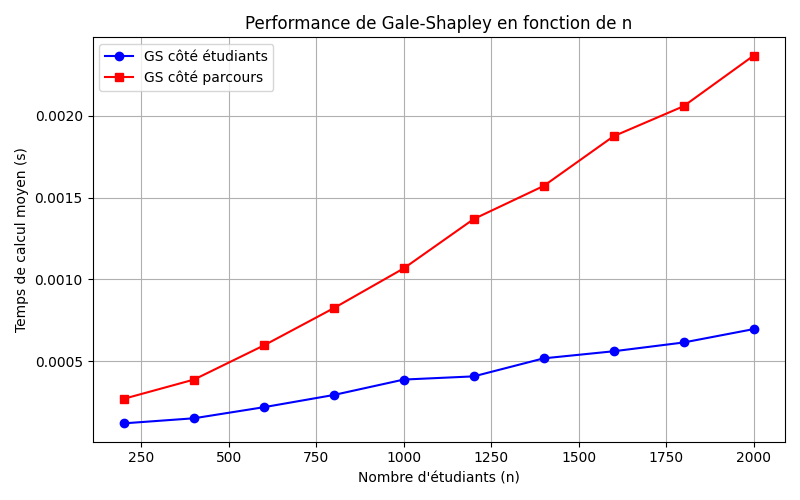
\includegraphics[width=0.85\linewidth]{performance_times.png}
  \caption{Temps de calcul moyen de Gale-Shapley (côté étudiants vs côté parcours) en fonction du nombre d'étudiants $n$, $m = 10$, capacités équilibrées, moyenne sur 10 tirages.}
  \label{fig:perf_times}
\end{figure}

On observe une croissance \textbf{linéaire} en $n$ pour les deux variantes, conformément à la théorie. À $n = 2\,000$, \GS{} côté parcours est $\approx 3{,}4\times$ plus lent ($2{,}27$ ms vs $0{,}67$ ms) malgré une complexité asymptotique inférieure -- l'overhead pratique vient du nombre de propositions $\approx 5\times$ supérieur.

\subsection{Nombre d'itérations}

La figure~\ref{fig:perf_iters} présente le nombre moyen d'itérations (propositions) effectuées par chacun des deux algorithmes.

\begin{figure}[h!]
  \centering
  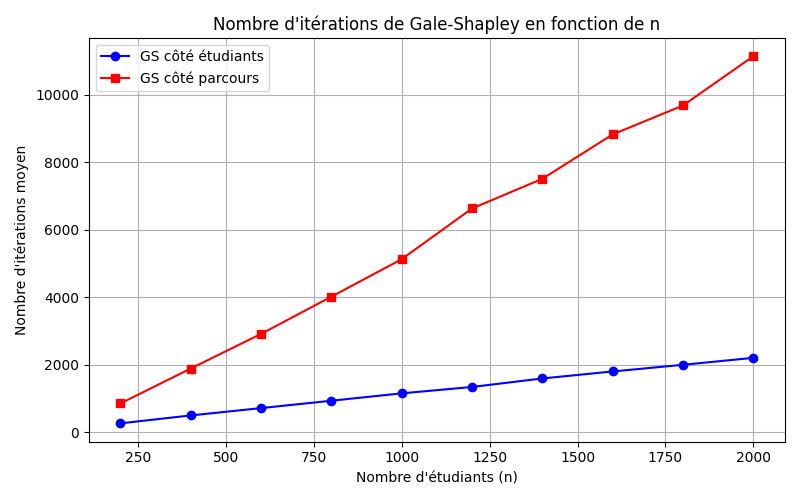
\includegraphics[width=0.85\linewidth]{performance_iters.png}
  \caption{Nombre d'itérations moyen de Gale-Shapley (côté étudiants vs côté parcours) en fonction du nombre d'étudiants $n$, $m = 10$, moyenne sur 10 tirages.}
  \label{fig:perf_iters}
\end{figure}

On observe également une croissance \textbf{linéaire} en $n$, bien en-deçà du pire cas $n \times m$. La version étudiants est nettement plus économique ($\approx 1{,}1n$ vs $5{,}4n$ propositions) car la max-heap évite les aller-retours superflus entre étudiants libres et parcours pleins.

\subsection{Conclusion}

\GS{} côté étudiants est plus efficace en pratique ; \GS{} côté parcours est conceptuellement plus simple ($O(1)$ par proposition) mais compense en volume. Pour des instances de grande taille avec peu de parcours ($m \ll n$), la version étudiants reste préférable.

\end{document}
